%TODO Still too short,
%TODO Calculate  primepaths in the last example and do the text cases.

\documentclass[handout]{beamer}
\usetheme{default}
\usepackage{tikz}
\usetikzlibrary{positioning}
\setbeamertemplate{footline}[page number]
\setbeamertemplate{navigation symbols}{}
\usepackage{hyperref}
\usepackage{listings}
\lstset{language=C}
\newcommand{\todo}[1]{{\tt ... #1 ... }}
\newcommand{\Reach}{\mathrm{Reach}}
\newcommand{\Path}{\mathrm{path}}

%Stolen from Stackexchange
%http://tex.stackexchange.com/questions/20609/strikeout-in-math-mode 
\newcommand\hcancel[2][red]{\setbox0=\hbox{$#2$}%
\rlap{\raisebox{.45\ht0}{\textcolor{#1}{\rule{\wd0}{1pt}}}}#2} 

\newcommand{\recordingpause}{
\begin{frame}{Recording Pause}
  \begin{center}
    Recording Pause
  \end{center}
\end{frame}
}
% \renewcommand{\recordingpause}{}

\title{Software Testing\\ Lecture 4\\ More about Coverage}
\author{Justin Pearson}
\date{2020}
%\setbeamertemplate{footline}[page number]
%\setbeamertemplate{navigation symbols}{}

\begin{document}
\lstset{language=C}

\begin{frame}
  \maketitle
\end{frame}

%\begin{frame}
%  \frametitle{Summary so far}
%  \begin{itemize}
%  \item Turing's halting theorem tells us in a strong sense that testing
%    for correctness is impossible.
%  \item Formalising programs as control flow graphs gives us a way to talk
%    about testing.
%  \item Node coverage corresponds to statement coverage, edge coverage
%    corresponds to something like branch coverage. Covering all execution
%    paths is impossible with loops, so there are various approximations.
%  \end{itemize}
%  Don't forget the distinction between syntactic and semantic reachability. 
%\end{frame}
%
%  \begin{frame}{Test Cases and Test Paths}
%\begin{center}
%   \begin{tikzpicture}
%     \node[rectangle,draw,fill=blue!20] (test1) {Test 1};
%     \node[rectangle,below of=test1,draw,fill=blue!20] (test2) {Test 2};
%     \node[rectangle,below of=test2,draw,fill=blue!20] (test3) {Test
%       3};
%     \node[right of=test2,node distance=10em]  (placementnode) {};
%     \node[rectangle,right of=placementnode,draw,fill=blue!20] (path)
%     {Test Path};
%     \draw [->] (test1) to (path);
%     \draw [->] (test2) to (path);
%     \draw [->] (test3) to (path);
%   \end{tikzpicture}
%\end{center}
%Many to one. Deterministic software, each test path has identical
%execution.
%\begin{center}
%   \begin{tikzpicture}
%     \node[rectangle,draw,fill=blue!20] (test1) {Test 1};
%     \node[rectangle,below of=test1,draw,fill=blue!20] (test2) {Test 2};
%     \node[rectangle,below of=test2,draw,fill=blue!20] (test3) {Test
%       3};
%     \node[rectangle,right of=test1,draw,fill=blue!20,node
%     distance=10em] (path1) {Test Path 1};
%     \node[rectangle,right of=test2,draw,fill=blue!20,node
%          distance=10em] (path2) {Test Path 2};
%     \node[rectangle,right of=test3,draw,fill=blue!20,node
%     distance=10em] (path3) {Test Path 3};
%     \draw[->] (test1) to (path1);
%     \draw[->] (test1) to (path2);
%     \draw[->] (test1) to (path3);
%     \draw[->] (test2) to (path1);
%     \draw[->] (test2) to (path2);
%     \draw[->] (test2) to (path3);
%     \draw[->] (test3) to (path1);
%     \draw[->] (test3) to (path2);
%     \draw[->] (test3) to (path3);
%   \end{tikzpicture}
%\end{center}
%Many to many, non-deterministic software (you'll meet it all the time)
%a test can execute many test paths.
%\end{frame}
%
\begin{frame}{Thinking about testing}
  Important to separate:
  \begin{itemize}
  \item What coverage criteria are we trying to test?
    \begin{itemize}
    \item Branch, statement, function points $\ldots$
    \end{itemize}
  \item How do we test this property?
    \begin{itemize}
    \item What paths do we cover in the control flow graph?
    \end{itemize}
    \item What test cases (inputs and expected outputs) will make the
      paths execute? 
  \end{itemize}
\end{frame}

 \begin{frame}{More material from the last lecture}
   \begin{itemize}
   \item Test path: represents the execution of a test case. It is a
     purely syntactic characterisation.  A test path might not be
     semantically possible.
   \item Test case design: separate out {\em Test Requirements}
     describe the theoretic properties of test paths, based on the
     graph; while {\em Test Criterion} is what we want the test
     requirement to do.
    \item The {\em Satisfaction} problem: given some test requirement how do I
      find or does my set of test paths satisfy the requirements. 
    \end{itemize}
    General idea in testing. Define your test requirements separately from the
    tests cases. Reformulate your requirements into test criteria and then try
    to find test paths that satisfy your test criteria.
\end{frame}




 \begin{frame}{Testing and Coverage of  Control Flow Graphs}
   \begin{itemize}
   \item {\em Test Requirements (TR)} : Describe properties of test paths.
     \item {\em Test Criterion} : Rules that define test requirements.
     \item {\em Satisfaction} : Given a set TR of test requirements
       for a criterion $C$, a set of tests $T$ satisfies C on a graph if
       and only if for every test requirement in TR, there is a test
       path in $\Path(T)$ that meets the test requirement.
   \end{itemize}
General idea in testing. Define your test requirements separately from
the tests cases. Reformulate your requirements  into test
criteria and then try to find test paths that satisfy your test
criteria.
 \end{frame}

\begin{frame}{Node Coverage --- Statement Coverage} 
  \begin{itemize}
  \item Node Coverage (NC) : Test set $T$ satisfies node coverage on
    graph $G$ iff for every syntactically reachable node $n$ in $N$, there
    is some path $p$ in path($T$) such that $p$ visits $n$.
  \end{itemize}
\end{frame}
\begin{frame}{Edge Coverage --- Branch Coverage}
  \begin{itemize}
  \item Edge Coverage (EC) : TR contains each reachable path of length
    up to 1, inclusive, in $G$.
  \end{itemize}
Is there any difference between node and edge coverage?
\end{frame}
\begin{frame}{Difference between node and edge coverage}
 \begin{columns}
   \begin{column}{0.5\textwidth}
     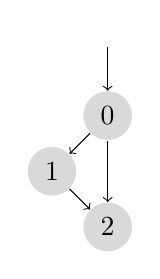
\begin{tikzpicture}
       \node (start) {};
       \node [below of=start,circle,fill=gray!30] (i) {$0$};
       \node [below left of=i,circle,fill=gray!30] (a) {$1$};
       \node [below right of=a,circle,fill=gray!30] (b) {$2$};
       \draw [->] (start) to (i);
       \draw [->] (i) to (a);
       \draw [->] (i) to (b);
       \draw [->] (a) to (b);
     \end{tikzpicture}
   \end{column}
   \begin{column}{0.5\textwidth}
     \begin{itemize}
     \item Node coverage
       \begin{itemize}
       \item Test requirement (TR) = $\{0,1,2\}$.
       \item Test path = $[0,1,2]$.
       \end{itemize}
     \item Edge Coverage
       \begin{itemize}
       \item Test requirement (TR) = $\{(0,1),(0,2),(1,2)\}$.
       \item Test paths = $[0,1,2],[0,2]$.
       \end{itemize}
     \end{itemize}
   \end{column}
 \end{columns}
\end{frame}

\recordingpause

\begin{frame}{Complete Path Coverage}
  \begin{itemize}
  \item Require that all paths are covered.
  \end{itemize}
  Often, there are too many paths. So you have to make an
  approximation, which is a comment theme in software testing.
  \begin{itemize}
  \item Require that all paths up to length $k$ are covered.
    \begin{itemize}
    \item $k=0$, node coverage.
    \item $k=1$, edge coverage.
    \item $k=2$, edge-pair coverage.
    \end{itemize}
  \end{itemize}
\end{frame}

 \begin{frame}{Structural Coverage Example}
  \begin{columns}
    \begin{column}{0.2\textwidth}
      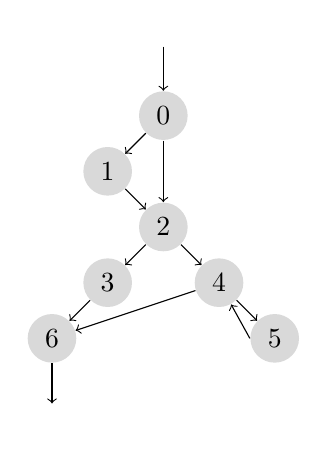
\begin{tikzpicture}
        \node (entry) {};
        \tikzstyle{every node} = [circle,fill=gray!30]
        \node[below of=entry] (a) {0};
        \node[below left of=a] (b) {1};
        \node[below right of=b] (c) {2};
        \node[below left of=c] (d) {3};
        \node[below right of=c] (e) {4};
        \node[below left of=d] (f) {6};
        \node[below right of=e] (g) {5};
        \node[draw=none,fill=none,below of=f] (exit) {};
        \draw[->] (entry) to (a);
        \draw[->] (a) to (b);
        \draw[->] (a) to (c);
        \draw[->] (b) to (c);
        \draw[->] (c) to (d);
        \draw[->] (c) to (e);
        \draw[->] (d) to (f);
        \draw[->] (e) to (f);
        \draw[->] (e) to (g);
        \draw[->] (g.west) to (e);
        \draw[->] (f) to (exit);
      \end{tikzpicture}
    \end{column}
    \begin{column}{0.8\textwidth}
      \begin{itemize}
      \item Node Coverage: $TR=\{0,1,2,3,4,5,6\}$, Test paths:
        $[0,1,2,3,6],[0,1,2,4,5,4,6]$.
      \item Edge Coverage:
        $TR=\{(0,1),(0,2),(1,2),(2,3),(2,4),(3,6),(4,5),(4,6), \newline (5,4)\}$,
        Test paths: $[0,1,2,3,6]$, $[0,2,4,5,4,6]$.
        % \item Edge-Pair Coverage:
        %   $TR=\{[0,1,2],[0,2,3],[0,2,4],[1,2,3],[1,2,4],[2,3,6],[2,4,5]$,$[2,4,6],[4,5,4],[5,4,5],[5,4,6]\}$.
      \item Complete Path Coverage. Test paths:
        $[0,1,2,3,6]$,$[0,1,2,4,6]$,$[0,1,2,4,5,4,6]$,
        $[0,1,2,4,5,4,5,4,6]$, etc.
      \end{itemize}
    \end{column}
  \end{columns}
\end{frame}

\begin{frame}{Structural Coverage Example}
  \begin{columns}
    \begin{column}{0.2\textwidth}
      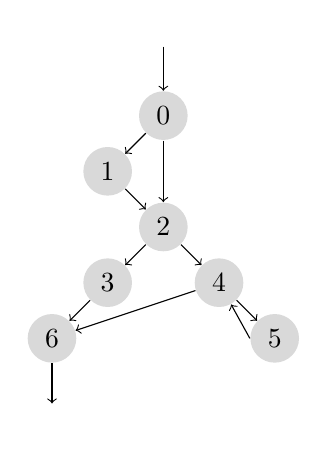
\begin{tikzpicture}
        \node (entry) {};
        \tikzstyle{every node} = [circle,fill=gray!30]
        \node[below of=entry] (a) {0};
        \node[below left of=a] (b) {1};
        \node[below right of=b] (c) {2};
        \node[below left of=c] (d) {3};
        \node[below right of=c] (e) {4};
        \node[below left of=d] (f) {6};
        \node[below right of=e] (g) {5};
        \node[draw=none,fill=none,below of=f] (exit) {};
        \draw[->] (entry) to (a);
        \draw[->] (a) to (b);
        \draw[->] (a) to (c);
        \draw[->] (b) to (c);
        \draw[->] (c) to (d);
        \draw[->] (c) to (e);
        \draw[->] (d) to (f);
        \draw[->] (e) to (f);
        \draw[->] (e) to (g);
        \draw[->] (g.west) to (e);
        \draw[->] (f) to (exit);
      \end{tikzpicture}
    \end{column}
    \begin{column}{0.8\textwidth}
      \begin{itemize}
      \item Edge-Pair Coverage: $TR=\{[0,1,2],[0,2,3]$,
        $[0,2,4],[1,2,3],[1,2,4]$,$[2,3,6]$, $[2,4,5]$,$[2,4,6]$,
        $[4,5,4],[5,4,5],[5,4,6]\}$
      \item Test Paths
        \begin{itemize}
        \item $[0,1,2,3,6]$,$[0,1,2,4,6]$, $[0,2,3,6]$
        \item $[0,2,4,5,4,5,4,6]$.
        \end{itemize}
      \end{itemize}
    \end{column}
  \end{columns}
\end{frame}


\begin{frame}{Loops}
There is a lot of theory, most of it is unsatisfactory. 
  \begin{itemize}
  \item Don't be content with branch coverage
  \item Look at your loops.
    \begin{itemize}
    \item Try to get them to execute zero times, once and many times.
    \end{itemize}
  \end{itemize}
\end{frame}
  \begin{frame}{Loops}
    \begin{itemize}
      
  \item If a graph contains a loop then it has an infinite number of
    paths.
  \item Thus you can not ask for complete path coverage. 
  \item Attempts to “deal with” loops:
    \begin{itemize}
    \item 1970s : Execute cycles once  ([4, 5, 4] in previous example, informal)
    \item 1980s : Execute each loop, exactly once (formalised)
    \item 1990s : Execute loops 0 times, once, more than once (informal description)
    \item 2000s : Prime paths
\end{itemize}
  \end{itemize}
  
\end{frame}
\recordingpause 
\begin{frame}{Simple and Prime Paths}
  \begin{itemize}
  \item A {\it path} is simple if no node appears more than once except
    possible that the first and last node can be the same. Note that this
    gives us unique edges.
  \item A {\it prime path} of a graph is a simple path that is not a
    sub-path of any other simple path.
  \end{itemize}
  
\end{frame}
\begin{frame}{Simple Paths}
\begin{columns}
%%%First Column    
\begin{column}{0.3\textwidth}    
 \tikzstyle{cfgnode}=[circle,fill=gray!30]
\begin{tikzpicture}%[node distance=1.5cm]
  \node (entry) {};
  \node[cfgnode,below of=entry] (a) {0};
  \node[below of=a] (middlenode) {};
  \node[cfgnode,left of=middlenode] (b) {1};
  \node[cfgnode,right of=middlenode] (c) {2};
  \node[cfgnode,below of=middlenode] (f) {3};
  \node[below of=f] (exit) {};
\draw[->] (entry) to (a);
\draw[->] (f) to (exit);
\draw[->] (f) to (a);
\draw[->] (a) to (b);
\draw[->] (a) to (c);
\draw[->] (b) to (f);
\draw[->] (c) to (f);
\end{tikzpicture}
\end{column}
%%%%Second Column
\begin{column}{0.6\textwidth}
  \begin{itemize}
  \item $[0]$,$[1]$,$[2]$,$[3]$
  \item $[0,1]$,$[0,2]$,$[1,3]$,$[2,3]$,$[3,0]$
  \item $[ 0,1,3]$, $[0,2,3]$, $[1,3,0]$, $[2,3,0]$,$[3,0,1]$
  \item $[ 0, 1, 3, 0 ]$, $[ 0, 2, 3, 0]$, $[ 1, 3, 0, 1 ]$,
$[ 2, 3, 0, 2 ]$, $[ 3, 0, 1, 3 ]$, $[ 3, 0, 2, 3 ]$, $[ 1, 3, 0, 2 ]$,
$[ 2, 3, 0, 1 ]$.
  \end{itemize}


\end{column}
\end{columns}
  
\end{frame}
\begin{frame}{Prime Paths}
  Remove all simple paths that can be extended (either direction) to a
  longer simple path.
\begin{columns}
%%%First Column    
\begin{column}{0.3\textwidth}    
 \tikzstyle{cfgnode}=[circle,fill=gray!30]
\begin{tikzpicture}%[node distance=1.5cm]
  \node (entry) {};
  \node[cfgnode,below of=entry] (a) {0};
  \node[below of=a] (middlenode) {};
  \node[cfgnode,left of=middlenode] (b) {1};
  \node[cfgnode,right of=middlenode] (c) {2};
  \node[cfgnode,below of=middlenode] (f) {3};
  \node[below of=f] (exit) {};
\draw[->] (entry) to (a);
\draw[->] (f) to (exit);
\draw[->] (f) to (a);
\draw[->] (a) to (b);
\draw[->] (a) to (c);
\draw[->] (b) to (f);
\draw[->] (c) to (f);
\end{tikzpicture}
\end{column}
%%%%Second Column
\begin{column}{0.6\textwidth}
  \begin{itemize}
  \item $\hcancel{[0]}$,$\hcancel{[1]}$,$\hcancel{[2]}$,$\hcancel{[3]}$
  \item $\hcancel{[0,1]}$,$\hcancel{[0,2]}$,$\hcancel{[1,3]}$,$\hcancel{[2,3]}$,$\hcancel{[3,0]}$
  \item $\hcancel{[ 0,1,3]}$, $\hcancel{[0,2,3]}$, $\hcancel{[1,3,0]}$, $\hcancel{[2,3,0]}$,$\hcancel{[3,0,1]}$
  \item $[ 0, 1, 3, 0 ]$, $[ 0, 2, 3, 0]$, $[ 1, 3, 0, 1 ]$,
$[ 2, 3, 0, 2 ]$, $[ 3, 0, 1, 3 ]$, $[ 3, 0, 2, 3 ]$, $[ 1, 3, 0, 2 ]$,
$[ 2, 3, 0, 1 ]$.
  \end{itemize}
In this case the prime paths are all the longest simple paths. Not
always the case. 
\end{column}
\end{columns}
  
\end{frame}
\begin{frame}{Prime Paths}
Enumerate all simple paths of length, 1,2,3, $\ldots$ then remove
simple paths that can be extended. You will be left with the prime paths.
\begin{columns}

\begin{column}{0.5\textwidth}
 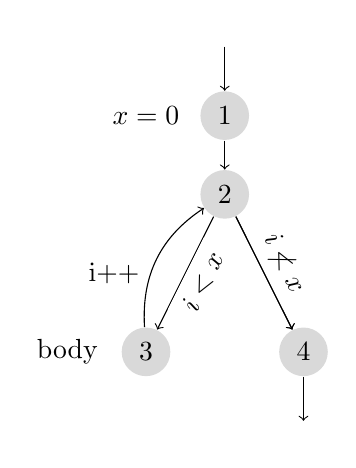
\begin{tikzpicture}
 \node (entry) at (1,3) {};
 
% \tikzstyle{every node} = [circle,fill=gray!30]
 \node[below of=entry,circle,fill=gray!30] (initialise) {$1$};
 \node[left  of=initialise] () {$x=0$};
 \node[below of=initialise,circle,fill=gray!30] (start) {$2$};
 \node[below of=start] (placementnode) {};
 \node[left of=placementnode, below of=placementnode,circle,fill=gray!30] (body)
 {$3$}; 
 \node[left of=body] () {body};
 \node[left of=placementnode,node distance=4em] (anchorpoint) {i++};
 \node[right of=placementnode, below of=placementnode,circle,fill=gray!30] (exit)
{$4$};
 \node[below of=exit] (exitnode) {};
 
 \draw [->] (exit) to (exitnode);
 \draw [->] (entry) to (initialise);
 \draw [->] (initialise) to (start);
 \draw [->] (start) --
 node[color=black,fill=white,pos=0.5,below,sloped] {$\scriptsize i<x$}
 (body);
 \draw [->] (start) --
 node[color=black,fill=white,pos=0.5,above,sloped] {$\scriptsize i\not<x$} (exit);
 \draw [->] (start) to (exit);
  \draw [->] (body) to[bend left] (start);
\end{tikzpicture}
\end{column}
%%%Second Column
\begin{column}{0.5\textwidth}
  \begin{itemize}
  \item $[1]$,$[2]$,$[3]$,$[4]$
  \item $[1,2]$, $[2,3]$, $[2,4]$, $[3,2]$
  \item $[1,2,3]$ , $[1,2,4]$, $[2,3,2]$, $[3,2,3]$,$[3,2,4]$
  \item We have to be careful about the paths of length 4.
    \begin{itemize}
    \item $[1,2,3,2]$ is not a simple path. Repeats $2$ which is not
      at the beginning or the end. 
    \end{itemize}
  \item In fact there are no simple paths of length 4 in this graph.
  \end{itemize}
\end{column}
\end{columns}
\end{frame}
%%%%%%%%%%
\begin{frame}{Prime Paths}
Enumerate all simple paths of length, 1,2,3, $\ldots$ then remove
simple paths that can be extended. You will be left with the prime paths.
\begin{columns}

\begin{column}{0.5\textwidth}
 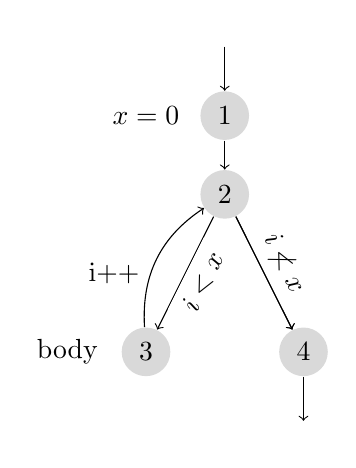
\begin{tikzpicture}
 \node (entry) at (1,3) {};
 
% \tikzstyle{every node} = [circle,fill=gray!30]
 \node[below of=entry,circle,fill=gray!30] (initialise) {$1$};
 \node[left  of=initialise] () {$x=0$};
 \node[below of=initialise,circle,fill=gray!30] (start) {$2$};
 \node[below of=start] (placementnode) {};
 \node[left of=placementnode, below of=placementnode,circle,fill=gray!30] (body)
 {$3$}; 
 \node[left of=body] () {body};
 \node[left of=placementnode,node distance=4em] (anchorpoint) {i++};
 \node[right of=placementnode, below of=placementnode,circle,fill=gray!30] (exit)
{$4$};
 \node[below of=exit] (exitnode) {};
 
 \draw [->] (exit) to (exitnode);
 \draw [->] (entry) to (initialise);
 \draw [->] (initialise) to (start);
 \draw [->] (start) --
 node[color=black,fill=white,pos=0.5,below,sloped] {$\scriptsize i<x$}
 (body);
 \draw [->] (start) --
 node[color=black,fill=white,pos=0.5,above,sloped] {$\scriptsize i\not<x$} (exit);
 \draw [->] (start) to (exit);
  \draw [->] (body) to[bend left] (start);
\end{tikzpicture}
\end{column}
%%%Second Column
\begin{column}{0.5\textwidth}
  \begin{itemize}
  \item $\hcancel{[1]}$,$\hcancel{[2]}$,$\hcancel{[3]}$,$\hcancel{[4]}$
  \item $\hcancel{[1,2]}$, $\hcancel{[2,3]}$, $\hcancel{[2,4]}$, $\hcancel{[3,2]}$
  \item $[1,2,3]$ , $[1,2,4]$, $[2,3,2]$, $[3,2,3]$
  \end{itemize}
\end{column}
\end{columns}
\end{frame}

%%%%%%%%%%
\begin{frame}{Prime Paths to Test Paths}
\begin{columns}

\begin{column}{0.5\textwidth}
 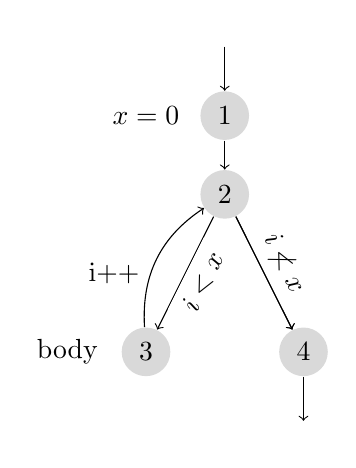
\begin{tikzpicture}
 \node (entry) at (1,3) {};
 
% \tikzstyle{every node} = [circle,fill=gray!30]
 \node[below of=entry,circle,fill=gray!30] (initialise) {$1$};
 \node[left  of=initialise] () {$x=0$};
 \node[below of=initialise,circle,fill=gray!30] (start) {$2$};
 \node[below of=start] (placementnode) {};
 \node[left of=placementnode, below of=placementnode,circle,fill=gray!30] (body)
 {$3$}; 
 \node[left of=body] () {body};
 \node[left of=placementnode,node distance=4em] (anchorpoint) {i++};
 \node[right of=placementnode, below of=placementnode,circle,fill=gray!30] (exit)
{$4$};
 \node[below of=exit] (exitnode) {};
 
 \draw [->] (exit) to (exitnode);
 \draw [->] (entry) to (initialise);
 \draw [->] (initialise) to (start);
 \draw [->] (start) --
 node[color=black,fill=white,pos=0.5,below,sloped] {$\scriptsize i<x$}
 (body);
 \draw [->] (start) --
 node[color=black,fill=white,pos=0.5,above,sloped] {$\scriptsize i\not<x$} (exit);
 \draw [->] (start) to (exit);
  \draw [->] (body) to[bend left] (start);
\end{tikzpicture}
\end{column}
%%%Second Column
\begin{column}{0.5\textwidth}
  \begin{itemize}
  \item $[1,2,3] \rightarrow [1,2,3,2,4]$ or $[2,3,2] \rightarrow [1,2,3,2,4]$
    \begin{itemize}
    \item Execute loop once.
    \end{itemize}
  \item $[1,2,4] \rightarrow [1,2,4]$
    \begin{itemize}
    \item   Execute loop zero times.
    \end{itemize}

  \item $[3,2,3] \rightarrow [1,2,3,2,3,2,4]$
    \begin{itemize}
    \item Execute loop more than once.
    \end{itemize}
  \end{itemize}
\end{column}
\end{columns}
\end{frame}
\begin{frame}{Simple Paths}
\begin{columns}
 \begin{column}{0.35\textwidth}
 \tikzstyle{cfgnode}=[circle,fill=gray!30]
 \begin{tikzpicture}
      \node[cfgnode] (g1) {1};
      \node[cfgnode,below=0.5cm of g1] (loopinit) {2};
      \node[cfgnode,below=0.5cm of loopinit] (loopbody) {3};
      \draw[->] (loopinit) to (loopbody);
      \node[cfgnode,below=0.5cm  of loopbody] (loopif) {4};
      \node[cfgnode,below left=1cm of loopif] (loopbodyifstatement) {5};
      \node[cfgnode,below=1cm of loopif] (loopbodyifelse) {6};
      \node[cfgnode,below=0.5cm  of loopbodyifelse] (returnstatment) {7};
      \draw[->] (g1) to (loopinit);
%      \draw[->] (loopbody) to (loopif);
      \path (loopbody) edge[->,above,pos=0.9]  (loopif);
      \draw[->] (loopif) to  (loopbodyifstatement);
      \draw[->] (loopif) to   (loopbodyifelse);
      \draw[->] (loopbodyifstatement) to (loopbodyifelse);
      \path (loopbodyifelse) edge[->,bend right=80,above]   (loopbody);
      \path (loopbody) edge[->,bend left=120,below,pos=0.6] (returnstatment);
\end{tikzpicture}
\end{column}
\begin{column}{0.65\textwidth}
  \begin{itemize}
  \item $[1]$, $[2]$, $[3]$,$[4]$,$[5]$,$[6]$,$[7]!$
  \item $[1,2]$,$[2,3]$,$[3,4]$,$[3,7]$, $[4,5]$,$[4,6]$,$[5,6]$,
    $[6,3]$,$[6,3]$
  \item $[1,2,3]$, $[2,3,4]$, $[2,3,7]!$, $[3,4,5]$, $[3,4,6]$,
    $[4,5,6]$, $[4,6,3]$, $[4,6,3]$, $[5,6,3]$, $[5,6,3]$, $[6,3,4]$
  \item $[1,2,3,4]$, $[1,2,3,7]!$, $[2,3,4,5]$, $[2,3,4,6]$,
    $[3,4,5,6]$, $[3,4,6,3]$, $[3,4,6,3]$ , $[4,5,6,3]$ ,$[6,3,4,5]$,
    $[4,5,6,3]$, $[4,6,3,4]$, $[5,6,3,4]$
  \item $[1,2,3,4,5]$, $[1,2,3,4,6]$, $[2,3,4,5,6]$,$[2,3,4,6,3]$,
    $[3,4,5,6,3]$ , $[3,4,5,6,3]$,
  \item $[1,2,3,4,5,6]$.
  \end{itemize}
\end{column}
\end{columns}
\end{frame}
\begin{frame}{Prime Paths}
\begin{columns}
 \begin{column}{0.35\textwidth}
 \tikzstyle{cfgnode}=[circle,fill=gray!30]
 \begin{tikzpicture}
      \node[cfgnode] (g1) {1};
      \node[cfgnode,below=0.5cm of g1] (loopinit) {2};
      \node[cfgnode,below=0.5cm of loopinit] (loopbody) {3};
      \draw[->] (loopinit) to (loopbody);
      \node[cfgnode,below=0.5cm  of loopbody] (loopif) {4};
      \node[cfgnode,below left=1cm of loopif] (loopbodyifstatement) {5};
      \node[cfgnode,below=1cm of loopif] (loopbodyifelse) {6};
      \node[cfgnode,below=0.5cm  of loopbodyifelse] (returnstatment) {7};
      \draw[->] (g1) to (loopinit);
%      \draw[->] (loopbody) to (loopif);
      \path (loopbody) edge[->,above,pos=0.9]  (loopif);
      \draw[->] (loopif) to  (loopbodyifstatement);
      \draw[->] (loopif) to   (loopbodyifelse);
      \draw[->] (loopbodyifstatement) to (loopbodyifelse);
      \path (loopbodyifelse) edge[->,bend right=80,above]   (loopbody);
      \path (loopbody) edge[->,bend left=120,below,pos=0.6] (returnstatment);
\end{tikzpicture}
\end{column}
\begin{column}{0.65\textwidth}
  \begin{itemize}
  \item $\hcancel{[1]}$, $\hcancel{[2]}$, $\hcancel{[3]}$,$\hcancel{[4]}$,$\hcancel{[5]}$,$\hcancel{[6]}$,$\hcancel{[7]!}$
  \item $\hcancel{[1,2]}$,$\hcancel{[2,3]}$,$\hcancel{[3,4]}$,$\hcancel{[3,7]}$, $\hcancel{[4,5]}$,$\hcancel{[4,6]}$,$\hcancel{[5,6]}$,
    $\hcancel{[6,3]}$,$\hcancel{[6,3]}$
  \item $\hcancel{[1,2,3]}$, $\hcancel{[2,3,4]}$, $\hcancel{[2,3,7]!}$, $\hcancel{[3,4,5]}$, $\hcancel{[3,4,6]}$,
    $\hcancel{[4,5,6]}$, $\hcancel{[4,6,3]}$, $\hcancel{[4,6,3]}$, $\hcancel{[5,6,3]}$, $\hcancel{[5,6,3]}$, $\hcancel{[6,3,4]}$
 \item $\hcancel{[1,2,3,4]}$, $[1,2,3,7]!$, $\hcancel{[2,3,4,5]}$, $\hcancel{[2,3,4,6]}$,
    $\hcancel{[3,4,5,6]}$,  $[3,4,6,3]$ , $\hcancel{[4,5,6,3]}$ ,$[6,3,4,5]$,
  $[4,6,3,4]$, $[5,6,3,4]$
  \item $\hcancel{[1,2,3,4,5]}$, $\hcancel{[1,2,3,4,6]}$,
    $\hcancel{[2,3,4,5,6]}$, $[3,4,5,6,3]$, 
  \item $[1,2,3,4,5,6]$.
  \end{itemize}
\end{column}
\end{columns}
\end{frame}

\begin{frame}{Prime Paths}
\begin{columns}
 \begin{column}{0.35\textwidth}
 \tikzstyle{cfgnode}=[circle,fill=gray!30]
 \begin{tikzpicture}
      \node[cfgnode] (g1) {1};
      \node[cfgnode,below=0.5cm of g1] (loopinit) {2};
      \node[cfgnode,below=0.5cm of loopinit] (loopbody) {3};
      \draw[->] (loopinit) to (loopbody);
      \node[cfgnode,below=0.5cm  of loopbody] (loopif) {4};
      \node[cfgnode,below left=1cm of loopif] (loopbodyifstatement) {5};
      \node[cfgnode,below=1cm of loopif] (loopbodyifelse) {6};
      \node[cfgnode,below=0.5cm  of loopbodyifelse] (returnstatment) {7};
      \draw[->] (g1) to (loopinit);
%      \draw[->] (loopbody) to (loopif);
      \path (loopbody) edge[->,above,pos=0.9]  (loopif);
      \draw[->] (loopif) to  (loopbodyifstatement);
      \draw[->] (loopif) to   (loopbodyifelse);
      \draw[->] (loopbodyifstatement) to (loopbodyifelse);
      \path (loopbodyifelse) edge[->,bend right=80,above]   (loopbody);
      \path (loopbody) edge[->,bend left=120,below,pos=0.6] (returnstatment);
\end{tikzpicture}
\end{column}
\begin{column}{0.7\textwidth}
  \begin{itemize}
  \item $[1,2,3,7]! \rightarrow  [1,2,3,7]$
    \begin{itemize}
    \item  Do the loop zero times.
    \end{itemize}
  \item $[3,4,6,3] \rightarrow   [1,2,3,4,6,3,7]$
    \begin{itemize}
    \item Do the loop once and do not do the {\tt if}
    \end{itemize}
  \item  $[6,3,4,5] \rightarrow   [1,2,3,4,6,3,4,5,6,3,7]$,
    \begin{itemize}
    \item Do the loop twice, once with the {\tt if}  and once without.
    \end{itemize}
  \item $[4,6,3,4] \rightarrow   [1,2,3,4,6,3,4,6,3,7]$
    \begin{itemize}
    \item Do the loop twice, both times without taking the {\tt if}.
    \end{itemize}
  \item $[5,6,3,4] \rightarrow   [1,2,3,4,5,6,3,4,6,3,7]$
    \begin{itemize}
    \item Do the loop twice, take the {\tt if} once and once without,
      other way round from the previous case.
    \end{itemize}
  \item $[3,4,5,6,3] \rightarrow [1,2,3,4,5,6,3,7]$, loop once with
    one {\tt if}.
  \end{itemize}
\end{column}
\end{columns}
\end{frame}

\begin{frame}{Prime Paths: Summary}
  \begin{itemize}
  \item Prime paths give you a good way of deriving a set of test
    cases that cover various combinations of loops and branches.
  \item There is no formal guarantee about {\it completeness}. As in all
    testing it just formalises a good compromise. 
  \end{itemize}

\end{frame}

\recordingpause

\begin{frame}{Model, define, and approximate}
  \begin{itemize}
  \item Model what you want to test.
  \item Define coverage criteria.
  \item If coverage criteria is undecidable or require too many test
    cases then approximate. 
  \end{itemize}
 \end{frame}
\begin{frame}{Separate test requirements and test cases}
  \begin{itemize}
  \item Have a reason for a test.
  \item Test requirements are the reasons for tests.
  \item You need to find satisfying test cases. 
  \end{itemize}
 
\end{frame}



\begin{frame}[fragile]{Example}
\begin{lstlisting}
  int count_spaces(char* str) {
   int length, i,count;
   count = 0;
   length = strlen(str);
   for(i=1; i<length; i++)  { 
     if(str[i] == ' ') { count++; }
   }

  }
\end{lstlisting}
  
\end{frame}

\begin{frame}[fragile]{First Divide into Basic Blocks}
 \tikzstyle{block}=[shape=rectangle,draw,text width=6cm]
  \begin{tikzpicture}
    \node[block] (a) {
       \verb+int count =0;+ \\
       \verb+length = strlen(str);+
      };
      \node[below=0.2cm of a] {\verb-for(i=1; i<length; i++)-};
      \node[below=0.5cm of a] {\verb-if(str[i] == ' ')-};

    \node[block,below= 1cm of a] (b) {
         \verb-count++;- 
      };
    \node[block,below=1cm  of b] (c) {
           \verb+return(count);+
      };
          
  \end{tikzpicture}
\end{frame}

\begin{frame}[fragile]{CFG}
 \tikzstyle{block}=[shape=rectangle,draw,text width=4cm]
 \tikzstyle{cfgnode}=[circle,fill=gray!30]
  \begin{tikzpicture}
    \node[block] (block1) {
       \verb+int count =0;+ \\
       \verb+length = strlen(str);+
      };
    \node[block,below= 1cm of block1] (block2) {
        \verb-count++;-
      };
    \node[block,below=1cm  of block2] (block3) {
           \verb+return(count);+
      };
      \node[below=0.2cm of block1] {\verb-for(i=1; i<length; i++)-};
      \node[below=0.5cm of block2] {\verb-if(str[i] == ' ')-};

      \node[cfgnode,right=2cm of block1] (g1) {1};
      \node[cfgnode,below=0.5cm of g1] (loopinit) {2};
      \node[cfgnode,below=0.5cm of loopinit] (loopbody) {3};
      \node[right=2cm of loopinit] (loopinitcode) {\verb+i=1+};
      \draw[->] (loopinit) to (loopbody);
      \draw[->] (loopinit) to (loopinitcode);
      \node[cfgnode,below=0.5cm  of loopbody] (loopif) {4};
      \node[cfgnode,below left=1cm of loopif] (loopbodyifstatement) {5};
      \node[cfgnode,below=1cm of loopif] (loopbodyifelse) {6};
      \node[cfgnode,below=0.5cm  of loopbodyifelse] (returnstatment) {7};
      \draw[->] (block1) to (g1);
      \draw[->] (block2) to (loopbodyifstatement);
      \draw[->] (block3) to (returnstatment);
      \draw[->] (g1) to (loopinit);
%      \draw[->] (loopbody) to (loopif);
      \path (loopbody) edge[->,above,pos=0.9] node {$i  < length$} (loopif);
      \draw[->] (loopif) -- node[sloped,above] {==} (loopbodyifstatement);
      \draw[->] (loopif) -- node[sloped,above] {$\neq$}  (loopbodyifelse);
      \draw[->] (loopbodyifstatement) to (loopbodyifelse);
      \path (loopbodyifelse) edge[->,bend right=80,above]  node {{\tt i++}} (loopbody);
      \path (loopbody) edge[->,bend left=120,below,pos=0.6] node
      {$i \not <length$} (returnstatment);
  \end{tikzpicture}

\end{frame}

\begin{frame}{Test Path}
  \begin{itemize}
  \item Remember a {\it test path} is a path that starts at an entry node
    and leaves at an exit node.
  \end{itemize}
  
\end{frame}
\begin{frame}[fragile]{Node Coverage}
 \tikzstyle{block}=[shape=rectangle,draw,text width=4cm]
 \tikzstyle{cfgnode}=[circle,fill=gray!30]
  \begin{tikzpicture}
    \node[block] (block1) {
       \verb+int count =0;+ \\
       \verb+length = strlen(str);+
      };
    \node[block,below= 1cm of block1] (block2) {
        \verb-count++;-
      };
    \node[block,below=1cm  of block2] (block3) {
           \verb+return(count);+
      };
      \node[below=0.2cm of block1] {\verb-for(i=1; i<length; i++)-};
      \node[below=0.5cm of block2] {\verb-if(str[i] == ' ')-};

      \node[cfgnode,right=2cm of block1] (g1) {1};
      \node[cfgnode,below=0.5cm of g1] (loopinit) {2};
      \node[cfgnode,below=0.5cm of loopinit] (loopbody) {3};
      \node[right=2cm of loopinit] (loopinitcode) {\verb+i=1+};
      \draw[->] (loopinit) to (loopbody);
      \draw[->] (loopinit) to (loopinitcode);
      \node[cfgnode,below=0.5cm  of loopbody] (loopif) {4};
      \node[cfgnode,below left=1cm of loopif] (loopbodyifstatement) {5};
      \node[cfgnode,below=1cm of loopif] (loopbodyifelse) {6};
      \node[cfgnode,below=0.5cm  of loopbodyifelse] (returnstatment) {7};
      \draw[->] (block1) to (g1);
      \draw[->] (block2) to (loopbodyifstatement);
      \draw[->] (block3) to (returnstatment);
      \draw[->] (g1) to (loopinit);
%      \draw[->] (loopbody) to (loopif);
      \path (loopbody) edge[->,above,pos=0.9] node {$i < length$} (loopif);
      \draw[->] (loopif) -- node[sloped,above] {==} (loopbodyifstatement);
      \draw[->] (loopif) -- node[sloped,above] {$\neq$}  (loopbodyifelse);
      \draw[->] (loopbodyifstatement) to (loopbodyifelse);
      \path (loopbodyifelse) edge[->,bend right=80,above]  node {{\tt i++}} (loopbody);
      \path (loopbody) edge[->,bend left=120,below,pos=0.6] node
      {$i \not <length$} (returnstatment);
      \node[shape=rectangle,draw,text width=3cm, below=1cm of block3] {$TR
        = \{1,2,3,4,5,6,7\}$, Test path is $[1,2,3,4,5,6,3,7]$};
  \end{tikzpicture}

\end{frame}
 

\begin{frame}{Grey box testing}
  \begin{itemize}
  \item Our test path $[1,2,3,4,5,6,3,7]$ requires the loop to execute
    exactly once and to detect one space. So we might try the test
    case ({\tt " "},1) but this won't work. Don't forget that {\tt
      i=1} in the loop body.
  \item Instead we have to use the  test case ({\tt "H "},1)
  \item Thinking about what the code should do, and trying to
    construct a test case corresponding to a path, we have uncovered a
    fault.
  \end{itemize}
  \end{frame}

\begin{frame}[fragile]{Edge Coverage}
 \tikzstyle{block}=[shape=rectangle,draw,text width=4cm]
 \tikzstyle{cfgnode}=[circle,fill=gray!30]
  \begin{tikzpicture}
    \node[block] (block1) {
       \verb+int count =0;+ \\
       \verb+length = strlen(str);+
      };
    \node[block,below= 1cm of block1] (block2) {
        \verb-count++;-
      };
    \node[block,below=1cm  of block2] (block3) {
           \verb+return(count);+
      };
      \node[below=0.2cm of block1] {\verb-for(i=1; i<length; i++)-};
      \node[below=0.5cm of block2] {\verb-if(str[i] == ' ')-};

      \node[cfgnode,right=2cm of block1] (g1) {1};
      \node[cfgnode,below=0.5cm of g1] (loopinit) {2};
      \node[cfgnode,below=0.5cm of loopinit] (loopbody) {3};
      \node[right=2cm of loopinit] (loopinitcode) {\verb+i=1+};
      \draw[->] (loopinit) to (loopbody);
      \draw[->] (loopinit) to (loopinitcode);
      \node[cfgnode,below=0.5cm  of loopbody] (loopif) {4};
      \node[cfgnode,below left=1cm of loopif] (loopbodyifstatement) {5};
      \node[cfgnode,below=1cm of loopif] (loopbodyifelse) {6};
      \node[cfgnode,below=0.5cm  of loopbodyifelse] (returnstatment) {7};
      \draw[->] (block1) to (g1);
      \draw[->] (block2) to (loopbodyifstatement);
      \draw[->] (block3) to (returnstatment);
      \draw[->] (g1) to (loopinit);
%      \draw[->] (loopbody) to (loopif);
      \path (loopbody) edge[->,above,pos=0.9] node {$i  < length$} (loopif);
      \draw[->] (loopif) -- node[sloped,above] {==} (loopbodyifstatement);
      \draw[->] (loopif) -- node[sloped,above] {$\neq$}  (loopbodyifelse);
      \draw[->] (loopbodyifstatement) to (loopbodyifelse);
      \path (loopbodyifelse) edge[->,bend right=80,above]  node {{\tt i++}} (loopbody);
      \path (loopbody) edge[->,bend left=120,below,pos=0.6] node
      {$i\not <length$} (returnstatment);
      \node[shape=rectangle,draw,text width=3cm, below=1cm of block3] {$TR
        = \{(1,2),(2,3),(3,4),(3,7),$, $(4,5),(4,6),(5,6),(6,3)\}$,
        Test paths are $[1,2,3,4,5,6,3,7]$, $[1,2,3,4,6,3,7]$, $[1,2,3,7]$};
  \end{tikzpicture}

\end{frame}
 
\begin{frame}{Test Cases}
  \begin{itemize}
  \item $[1,2,3,4,5,6,3,7]$  ({\tt " "},1)
  \item $[1,2,3,4,6,7]$    ({\tt "H"},0)
  \item $[1,2,3,7]$       ({\tt ""},0)
  \end{itemize}
  \end{frame}

\recordingpause

\begin{frame}{Relaxing test cases}
  \begin{itemize}
  \item As we have seen, sometimes we have infeasible test cases.
    \begin{itemize}
    \item This might be because there is a fault.
    \item Or, that we have to do other things to get to the
      code. There might be a bit of setup code that we have to call
      first that is not in our path.
    \end{itemize}
  \item A path $p$ tours the path $s$ if $s$ is a sub-sequence of $p$.
    \begin{itemize}
    \item $[1,2,3,4,6,3,4,6,3,7]$ tours  the test path $[1,2,3,4,6,3]$ it
      also tours many other paths including $[4,6,3,7]$. 
    \item Don't forget the difference between a {\it test path} and a {\it path}.
    \end{itemize}
  \end{itemize}
    
\end{frame}
\begin{frame}{Relaxing Test Cases}
  \begin{itemize}
  \item A {\it test path} $p$ is set to {\em tour} sub-path $q$ with {\em
      side-trips} if every edge that is in $q$ is also in $p$ in the
    same order.
  \item A {\it test path} $p$ is set to {\em tour} sub-path $q$ with {\em
      detours} if every node that is in $q$ is also in $p$ in the
    same order.
  \end{itemize}
  
\end{frame}
\begin{frame}{Sidetrips}
 \tikzstyle{cfgnode}=[circle,fill=gray!30]
\begin{tikzpicture}[node distance=1.5cm]
  \node (entry) {};
  \node[cfgnode,right of=entry] (a) {0};
  \node[cfgnode,right of=a] (b) {1};
  \node[cfgnode,right of=b] (c) {2};
  \node[cfgnode,right of=c] (d) {4};
  \node[cfgnode,right of=d] (e) {5};
  \node[cfgnode,below of=c] (f) {3};
  \node[right of=e] (exit) {};
  \draw[->] (entry) to (a);
  \draw[->] (a) to (b);
  \draw[->] (b) to (c);
  \draw[->] (c) to (d);
  \draw[->] (d) to (e);
  \draw[->] (e) to (exit);
  \draw[->,bend left=45] (c) to (f);
  \draw[->,bend left=45] (f) to (c);
  \draw[->,bend right=45] (f.east) to (d);
\end{tikzpicture}
  
The path $[0,1,2,3,2,4,5]$ tours the path $[0,1,2,4,5]$ a side trip.
\end{frame}

\begin{frame}{Detours}
 \tikzstyle{cfgnode}=[circle,fill=gray!30]
\begin{tikzpicture}[node distance=1.5cm]
  \node (entry) {};
  \node[cfgnode,right of=entry] (a) {0};
  \node[cfgnode,right of=a] (b) {1};
  \node[cfgnode,right of=b] (c) {2};
  \node[cfgnode,right of=c] (d) {4};
  \node[cfgnode,right of=d] (e) {5};
  \node[cfgnode,below of=c] (f) {3};
  \node[right of=e] (exit) {};
  \draw[->] (entry) to (a);
  \draw[->] (a) to (b);
  \draw[->] (b) to (c);
  \draw[->] (c) to (d);
  \draw[->] (d) to (e);
  \draw[->] (e) to (exit);
  \draw[->,bend left=45] (c) to (f);
  \draw[->,bend left=45] (f) to (c);
  \draw[->,bend right=45] (f.east) to (d);
\end{tikzpicture}
  
The path $[0,1,2,3,4,5]$ tours the path $[0,1,2,4,5]$ with a detour.
\end{frame}
\begin{frame}{Infeasible  test requirements}
  \begin{itemize}
  \item An infeasible test requirement {\em cannot be satisfied}
    \begin{itemize}
    \item Unreachable statement (dead code)
    \item Can only be executed if a contradiction occurs $X>0 \land
      X<0$.
    \item Always check against the specification, it could be a fault. 
    \end{itemize}
  \end{itemize}
  
\end{frame}
\begin{frame}{Infeasible  test requirements}
  \begin{itemize}
  \item   Most test criteria have some infeasible test requirements. 
  \item It is usually undecidable if all test requirements
    are feasible (halting problem again).
  \item Allowing side trips might weaken the test cases, but allows
    more feasible test cases.
  \item Practical recommendation, best effort touring. Allow as many
    as possible without side-trips; only allow side-trips on
    infeasible test paths.
  \end{itemize}

  
\end{frame}




\begin{frame}
  \frametitle{Summary}

  \begin{itemize}
  \item  Prime paths provide some intuition for test cases for loops.
  \item  With nested loops and complicated branching, prime-paths give
    us test cases that you might not look for.
  \item There are various ways of relaxing test paths when they are infeasible.
  \end{itemize}
\end{frame}

\begin{frame}
  \frametitle{Do I expect you to draw control flow graphs?}
  \begin{itemize}
  \item For the exam yes. 
  \item But, why bother? For large pieces of code you will never bother. For
    troublesome small bits of code, {\it prime paths} would be a useful tool to look
    for test cases you might not consider.
  \item Formalisation allows you to think about what coverage means for a
    piece of code.
  \end{itemize}
  %%
\end{frame}
\end{document}

%%% Local Variables:
%%% mode: latex
%%% TeX-master: t
%%% End:
